\noindent
\subsubsection{Author based features}
\label{author_analysis}

We next look into some of the author based features like author reputation and author productivity to determine how they influence the long-term citation of the paper.  
\begin{figure*}
\centering
\begin{tabular}{ccc}
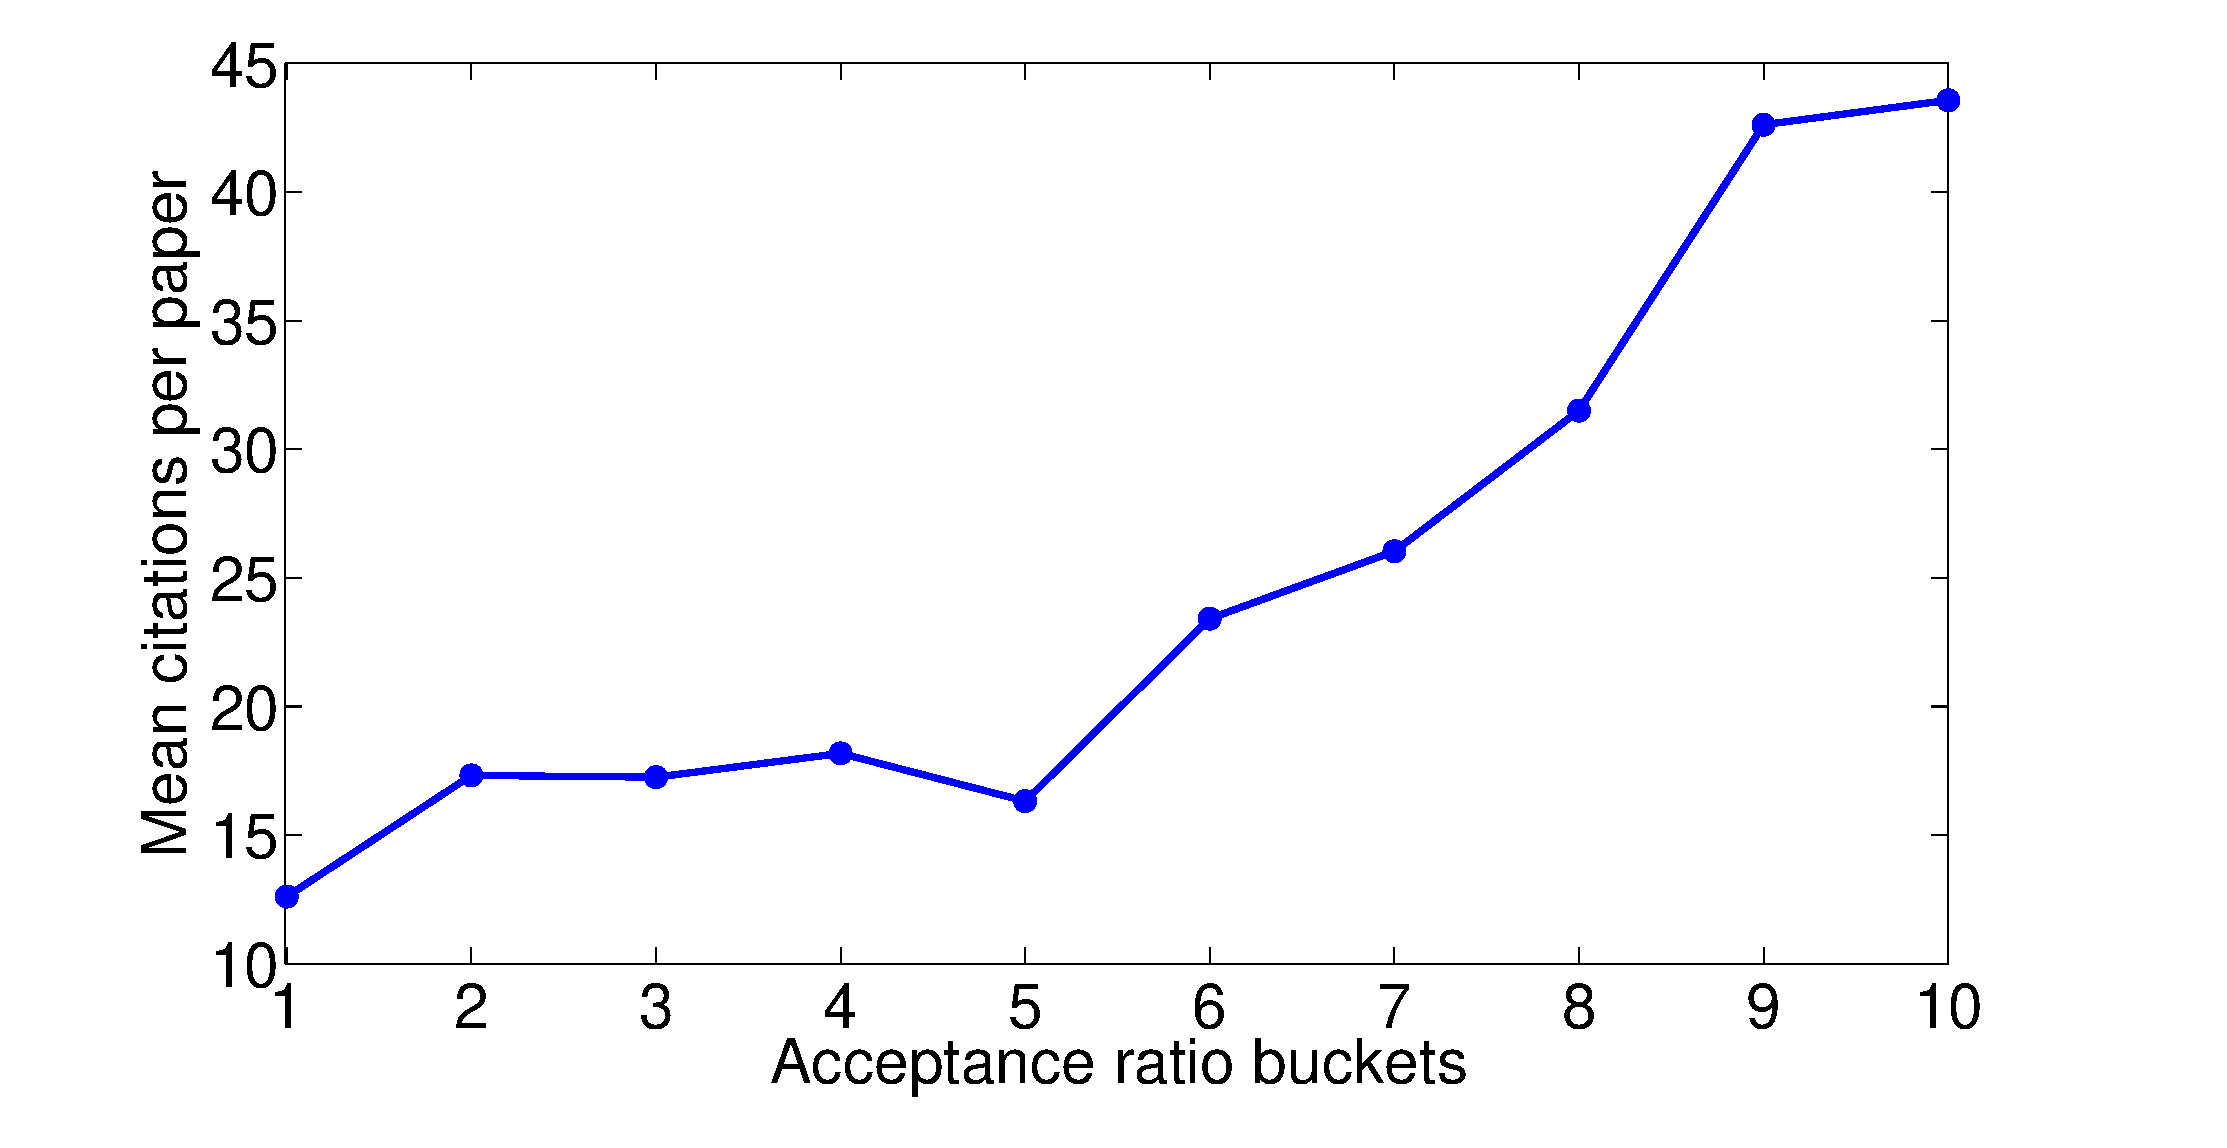
\includegraphics[scale=0.12]{./texfiles/Chapter_4/jcdl/figures/citation_succes_ratio.eps} & 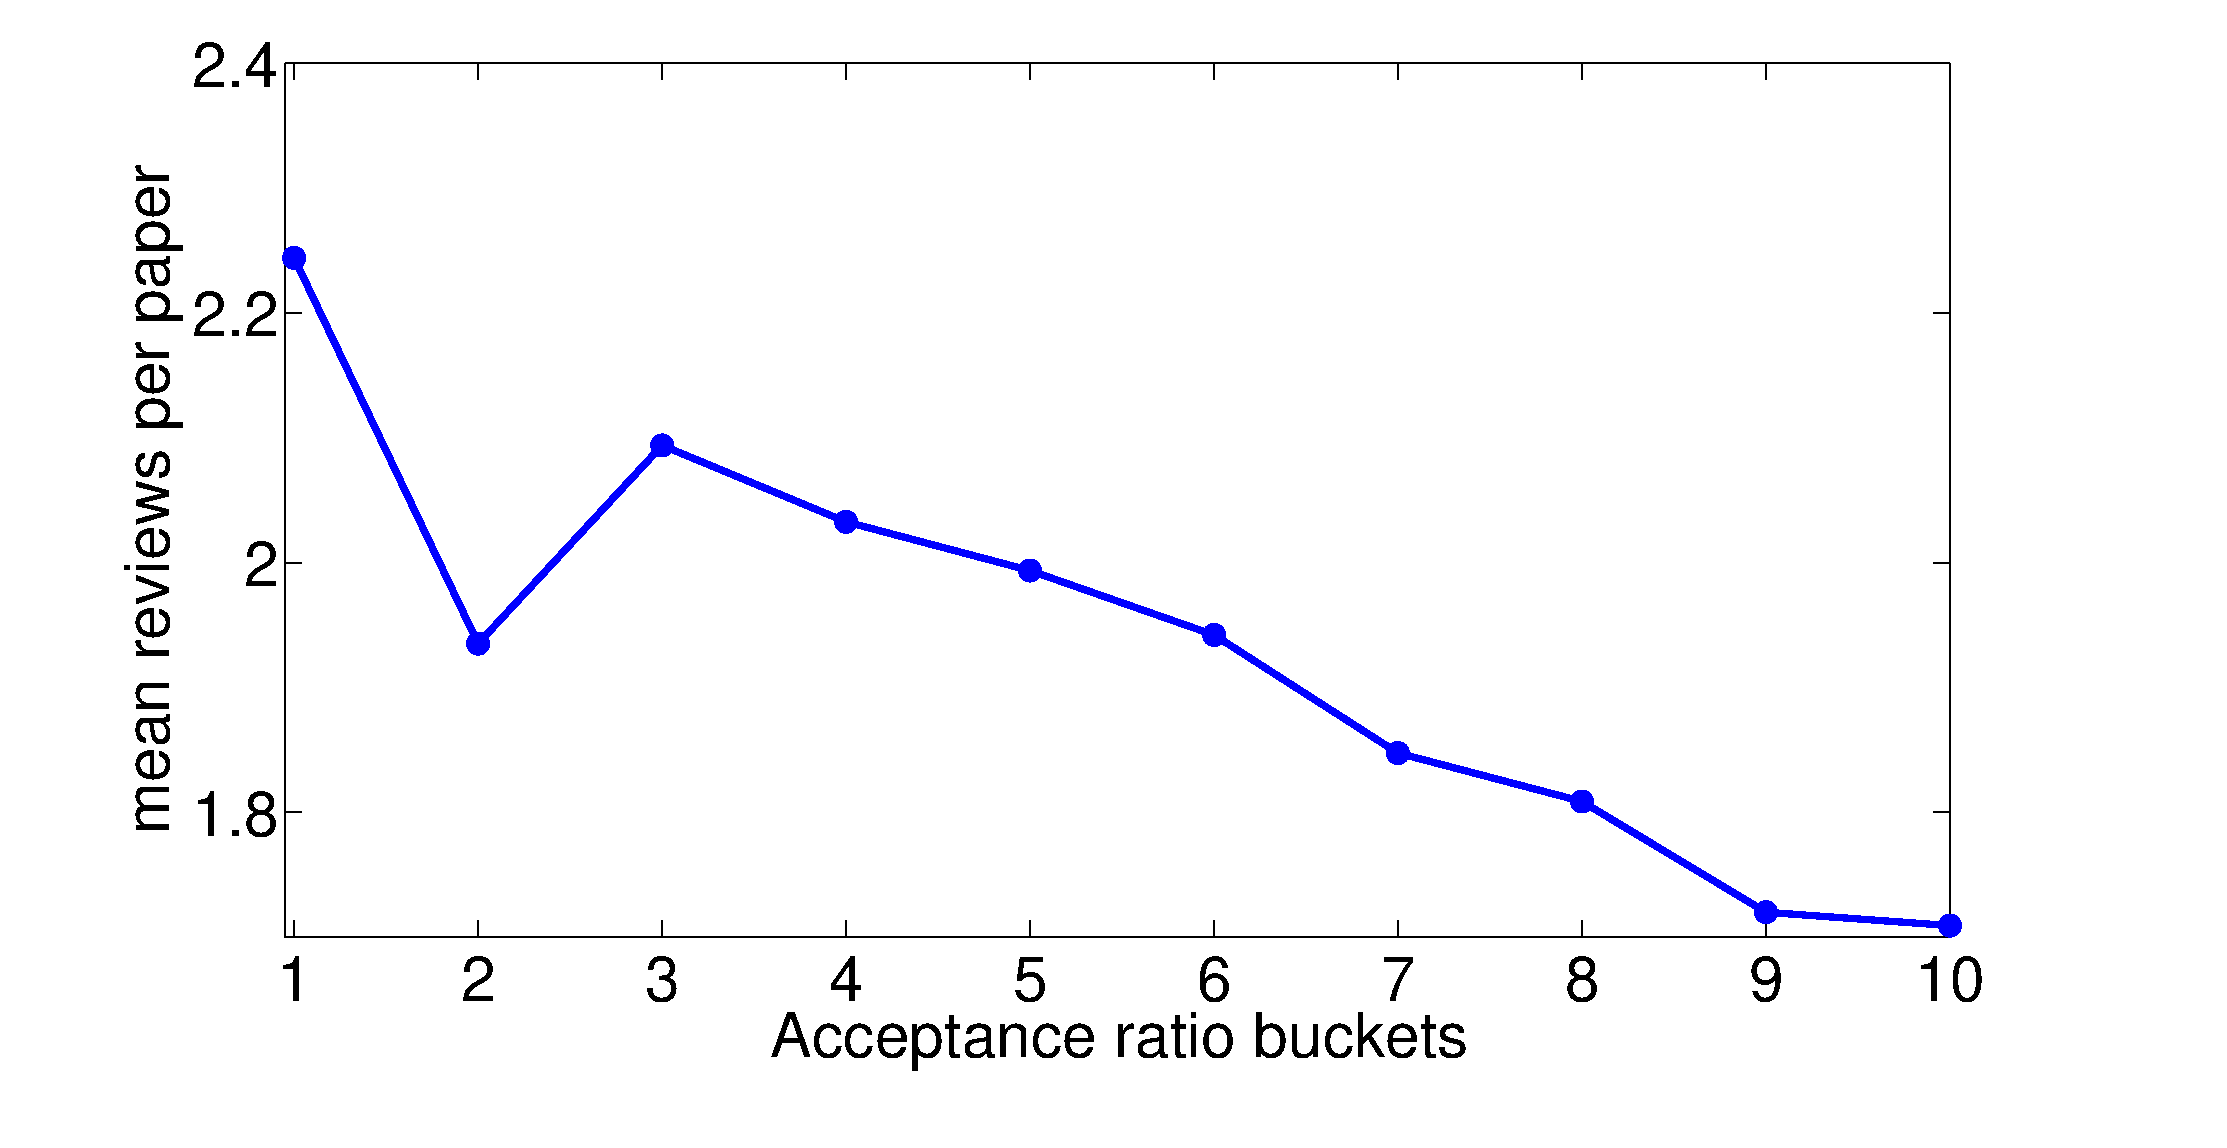
\includegraphics[scale=0.15]{./texfiles/Chapter_4/jcdl/figures/review_succes_ratio.eps} & 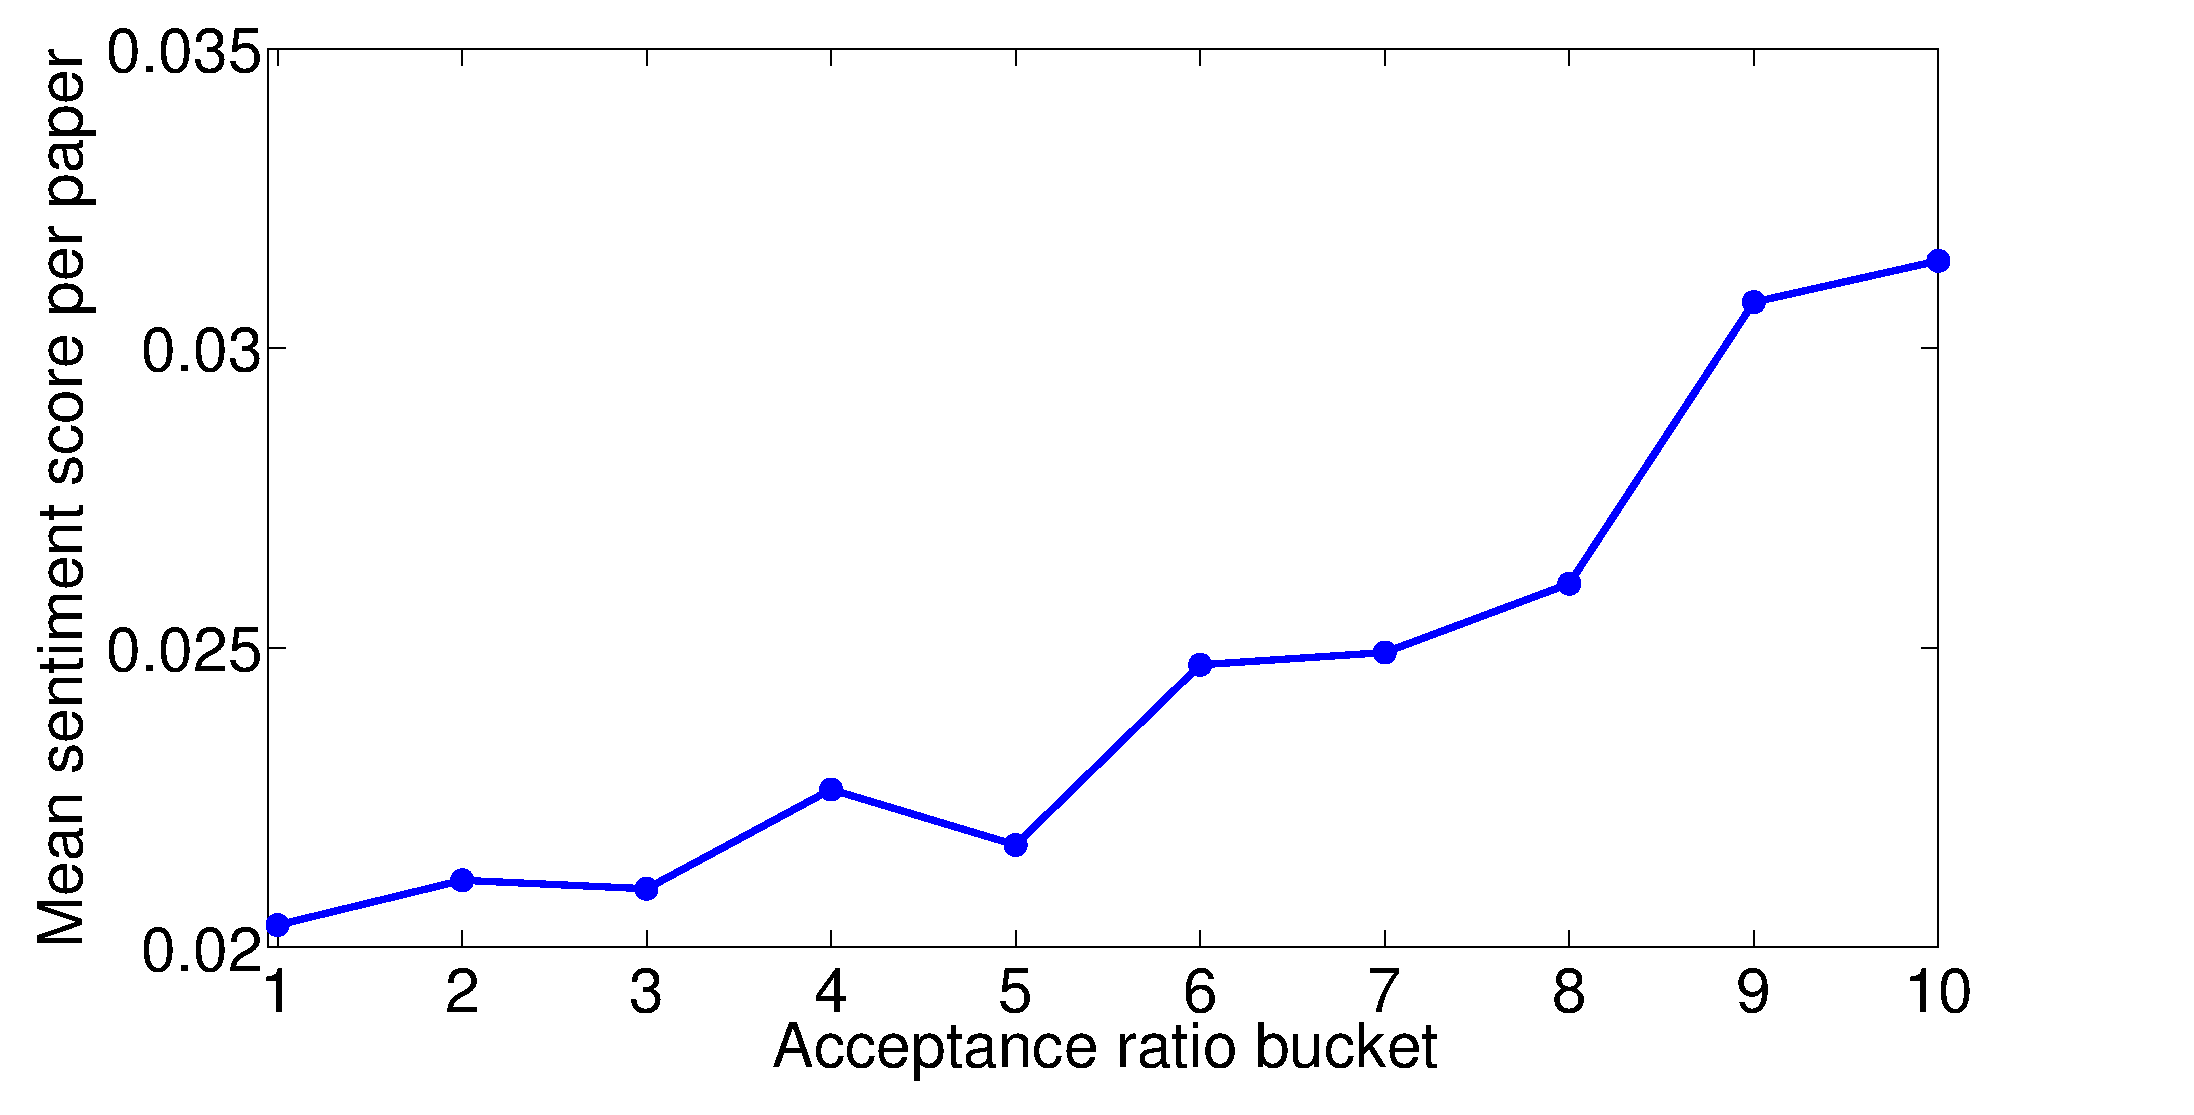
\includegraphics[scale=0.15]{./texfiles/Chapter_4/jcdl/figures/sentiment_succes_ratio-eps-converted-to.pdf}
\end{tabular}
\caption{{\bf (Left)} Mean number of citations per paper versus acceptance ratio. {\bf (Middle)} Mean number of reviews per paper versus acceptance ratio. {\bf (Right)} Mean sentiment score per paper versus acceptance ratio. Note that in each case we use acceptance ratio buckets where buckets correspond to acceptance ratio ($\geq 0.1$ and $< 0.2$), ($\geq 0.2$ and $<0.3$) and so on.}
\label{fig13}
\end{figure*}
\subsubsection*{Author reputation (AR)} We analyze whether there are some specific authors whose papers always get accepted and similarly there are others whose papers always get rejected.  
For each author we define a metric called {\bf acceptance ratio} which is the fraction of submitted papers accepted in JHEP. Formally, acceptance ratio of an author $i$ is defined by: $acceptance\,ratio_{i}=\frac{accept_{i}}{accept_{i} + reject_{i}}$.    
where $accept_{i}$ and $reject_{i}$ represents respectively the number of accepted and rejected papers of the author $i$ in JHEP. We use this metric as a proxy for author reputation.
We observe that mean acceptance ratio across all the authors is $0.56$. In fact, for almost 7\% of the authors, the acceptance ratio is 1. Next we check whether the authors with high acceptance ratio have higher citations per paper. To this aim we segregate authors based on the acceptance ratio and calculate the mean number of citations per paper for these authors (refer to figure~\ref{fig13}{\bf (Left)}). We observe an increasing trend suggesting that the authors with higher acceptance ratio tend to have higher citations. 
\iffalse
\begin{figure}
\centering
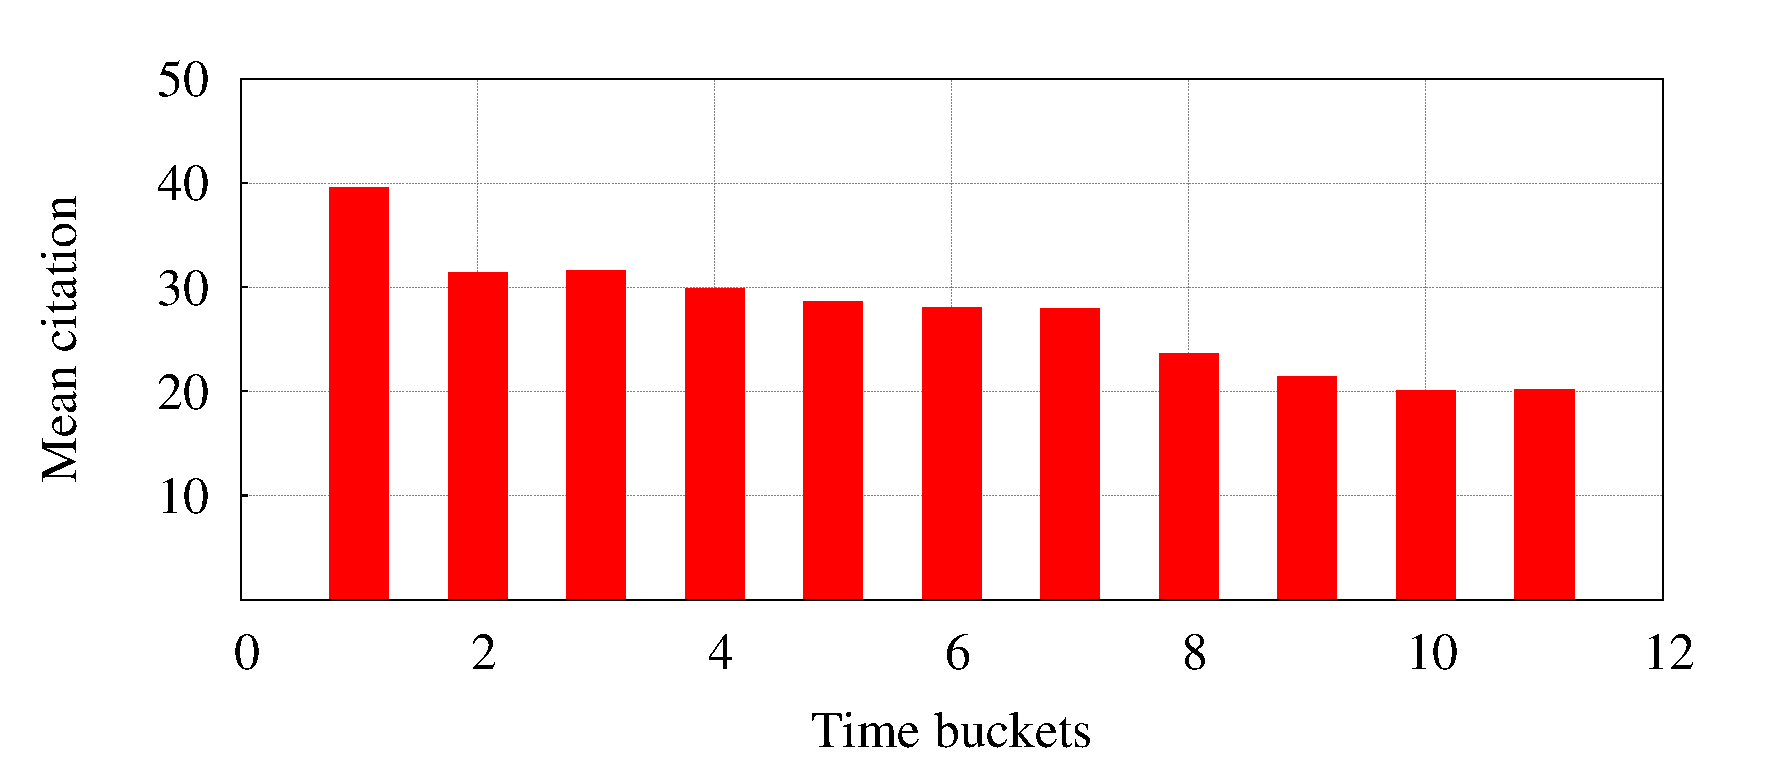
\includegraphics[scale=0.25]{./texfiles/Chapter_4/jcdl/figures/prod_citation.eps}
\caption{Mean citation of the papers versus the average time(in days) between two submission. Note that  we use time buckets where buckets correspond to $<100$,($\geq 100$ and $< 200$), ($\geq 200$ and $<300$) and so on.\vspace{-2mm}}
\label{fig:prod}
\end{figure}
\fi
To check whether the authors having higher acceptance ratio are also reviewed less, we again segregate the authors based on the acceptance ratio and calculate the average number of reviews received per paper for these authors (refer to figure~\ref{fig13}{\bf (Middle)}). We observe a decreasing trend implying that papers of authors with higher acceptance ratio are indeed reviewed less. Although there are authors with high acceptance ratio whose papers are reviewed less, they are often highly cited indicating the overall effectiveness of the review process. We further study the sentiment score of the review reports for authors with different acceptance ratios. For authors in a given  acceptance ratio bucket we calculate the average sentiment score of the review reports of their papers.
We observe that the authors having higher acceptance ratios tend to have more positive reviews on average compared to the others with lower acceptance ratios which is indicated by the increasing trend in the curve in figure~\ref{fig13}{\bf (Right)}. 

\subsubsection*{Author productivity (AP)} It is established in the literature \cite{yan2012better} that the more papers an author publishes, more are his chances of getting cited. We hence use it as a feature in predicting the long-term citation of the paper. We calculate for each author the mean time ($s_t$) between two submissions. We use $s_t$ as proxy for author productivity as low $s_t$ would indicate higher productivity rate and vice versa.  
The papers are segregated based on the corresponding author's $s_t$ and then the mean citation is calculated. Each bucket correspond to $<100$,($\geq 100$ and $< 200$), ($\geq 200$ and $<300$) and so on. We observe that more frequent the submission, more is the chance of getting citation (refer to figure \ref{fig:prod}).

\begin{figure}
\centering
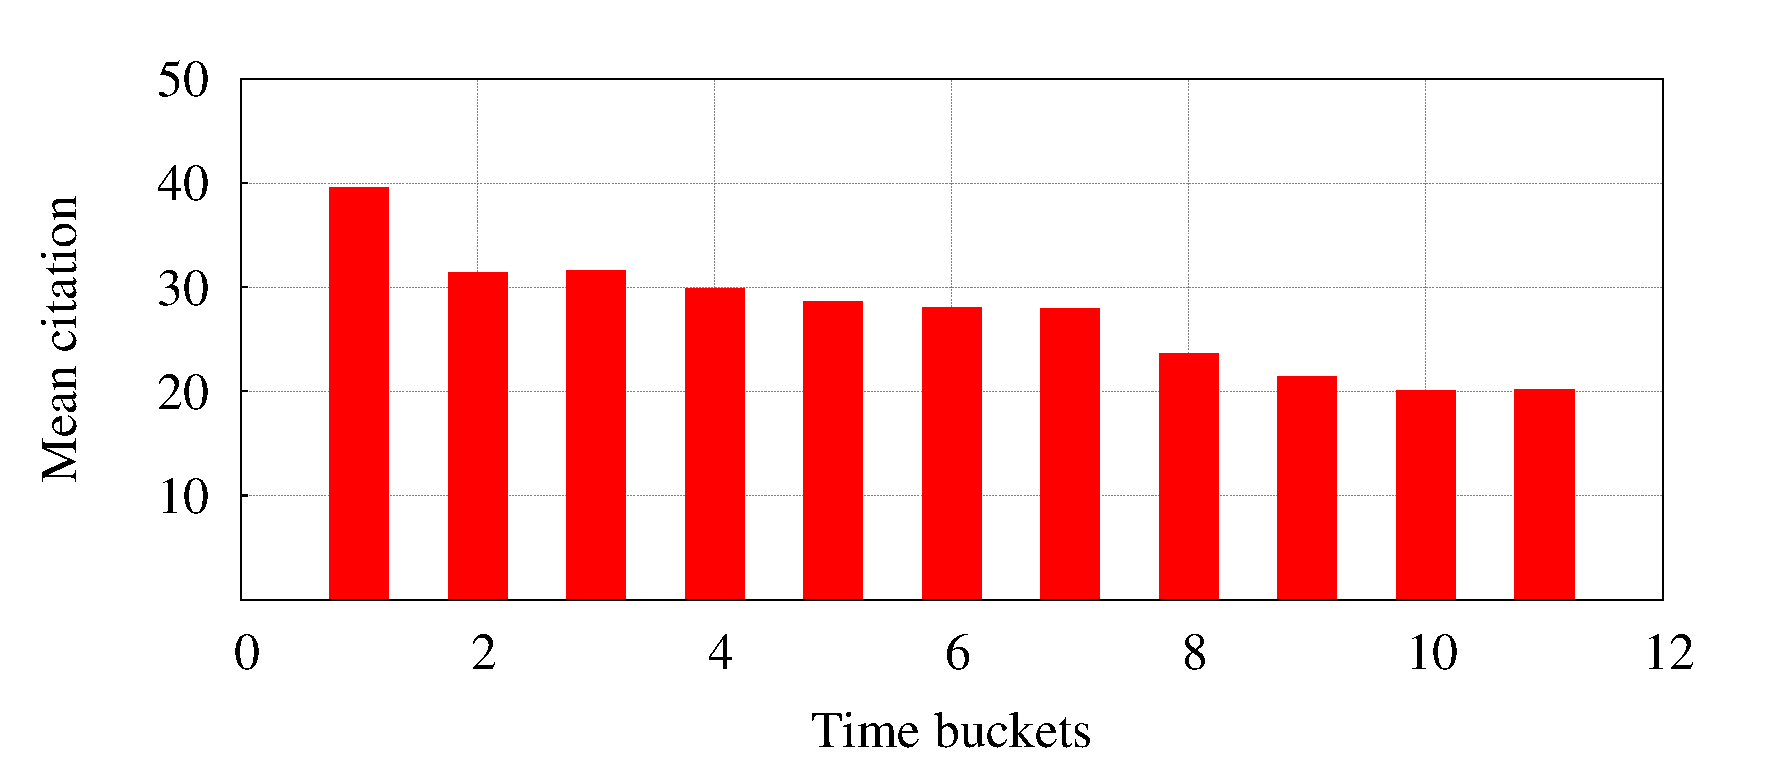
\includegraphics[scale=0.25]{./texfiles/Chapter_4/jcdl/figures/prod_citation.eps}
\caption{Mean citation of the papers versus the average time(in days) between two submission. Note that  we use time buckets where buckets correspond to $<100$,($\geq 100$ and $< 200$), ($\geq 200$ and $<300$) and so on.\vspace{4mm}}
\label{fig:prod}
\end{figure}

\subsection*{Influence of contributory authors on overall impact}

We now proceed to investigate the influence of contributory authors on the long term impact of the paper. In specific we look into eight different attributes (we elaborate on each of them next) which are aimed at measuring the prominence of the author and we intend to find whether most prominent or the least prominent author influences the long term impact of the paper. To complete the analysis we further consider the average values of the attributes as well. Note that all these attributes are calculated based on the submission history of the author at the time of the current submission. 

\noindent{\bf (1) Submissions (AS): }We consider for each contributory author the number of submissions (s)he has made prior to this submission. We argue that more the number of submissions, more mature the author and vice versa. 

\noindent{\bf (2) Citations (AC): }We next calculate for each author the average citations on his (her) prior submissions. Clearly the higher the citation more prominent the authors.

\noindent{\bf (3) Submission frequency (AF): }This is similar to the productivity metric defined previously. Here we calculate productivity of each author prior to the submission  

\noindent{\bf (4) Age: } We calculate age for each author as the time difference in number of days between his (her) first submission to the journal and the date of the current submission. This also roughly estimates the maturity of the author as higher the age more mature the author.

\noindent{\bf (5) Acceptance ratio (AAR): }That acceptance ratio is a measure of reputation for an author has been demonstrated earlier in this section and we use it in this task as well. Note that we measure the acceptance ratio from his (her) submission history prior to submission in question. 

\noindent{\bf (6) Collaborator diversity (ACD): }We further consider the diversity of each author's previous collaborators. We hypothesize that more diverse the set of previous collaborators, more reputed the author. To calculate the diversity we use entropy.

\noindent{\bf (7) Collaboration age (ACA): }For each contributing author we calculate the average age of his (her) collaborators in prior submissions. We argue that higher the average collaborator age, more prominent the author. 

\noindent{\bf (8) Topic diversity (ATD): }Although explicit topics are not available for a paper, the publisher does assign a set of keywords (between 2 and 4) to each submission which we use as proxy for topics. For each author we consider all the keywords associated with his (her) previous submissions and calculate entropy which is assigned as the diversity score of the author.

Given a submission we calculate all the above attributes for each contributing author and form three vectors consisting of the most reputed coauthor (i.e., a vector of the maximum values of the above attributes), least reputed coauthor (i.e., a vector of minimum values of the above attributes) and average (i.e., a vector of the average values of the above attributes). To determine each attributes' correlation with long term citation of a paper we perform the following exercise - 
\begin{enumerate}
 \item We segregate the papers based on the number of citations they have accrued. The bin sizes are of increasing power of 2 ($\leq 1$, 2, \{$> 2$ and $\leq 4$\} and so on).
 \item For each bin we calculate the mean of maximum (most reputed), minimum (least reputed) and average value of the attribute across all the papers.
\end{enumerate}


In figure \ref{fig:author}(a) and \ref{fig:author}(b) we present the results for (i) submissions and (ii) collaborator diversity respectively. We observe an increasing trend when we consider the maximum values or the most reputed coauthors while no such obvious pattern is observed in case of the minimum values or the least reputed coauthor. The above observation indicates that the most reputed coauthor has the maximum influence in driving the long term citation of the paper. We observe similar results for other attributes as well. 

\begin{figure}
\centering
\includegraphics[scale=0.25]{./texfiles/Chapter_4/jcdl/figures/author_features.eps}
\caption{Mean of maximum (most reputed), minimum (least reputed) and average value of (a) submissions and (b) collaboration diversity for a given citation bin. The bin sizes are of increasing power of 2 ($\leq 1$, 2, \{$> 2$ and $\leq 4$\} and so on).\vspace{4mm}}
\label{fig:author}
\end{figure}

%\medskip